\documentclass{beamer}
\usepackage[utf8]{inputenc}
\usepackage[russian]{babel}
\usepackage[T2A]{fontenc}
\usepackage{amsmath}
\usepackage{amsfonts}
\usepackage{amsthm}
\usepackage{bbm}
\usepackage{amssymb}
\usepackage{bm}
\usepackage{graphicx}
\usepackage{epstopdf}
\usepackage[]{algorithm2e}
\usepackage{amsthm}

%\usetheme{Warsaw}
%\usecolortheme{sidebartab}
\usetheme{Warsaw}
\usecolortheme{seahorse}

%\definecolor{beamer@blendedblue}{RGB}{255,255,0}
%\definecolor{beamer@blendedblue}{HTML}{008A34} %green
%\definecolor{beamer@blendedblue}{HTML}{4A4A4A} %grey
%\definecolor{beamer@blendedblue}{HTML}{0E9059} %biryuz
\definecolor{beamer@blendedblue}{HTML}{027466} %blue


\theoremstyle{definition}
\newtheorem{defin}{Definition}
\newtheorem{assumption}{Assumption}
\theoremstyle{plain}
\newtheorem{thm}{Theorem}
\newtheorem{lem}{Lemma}
\newtheorem{prop}{Proposition}
\theoremstyle{remark}
\newtheorem{remark}{Remark}
\newtheorem{prob}{Problem}
\def\eqdef{\stackrel{def}{=}}

% \DeclareMathOperator*{\argmin}{argmin} 
% \DeclareMathOperator*{\Argmin}{Argmin} 
% \DeclareMathOperator{\barcnt}{bar}
% \DeclareMathOperator{\supp}{supp}
% \DeclareMathOperator{\est}{\mathbb{E}}
% \DeclareMathOperator{\inter}{int}
% \DeclareMathOperator{\ind}{Ind}

\begin{document}
\setlength{\abovedisplayskip}{5pt}
\setlength{\belowdisplayskip}{5pt}

	\title[\hbox to 60mm{Course project \hfill\insertframenumber\,/\,20}]
			{ Course project \\ <<Optimization approaches to community detection>>}
	\author[Igor Silin]{\large Marina Danilova, Alexander Podkopaev, Nikita Puchkin, Igor Silin}
	\institute[Affiiation]{
	\textsc{Skolkovo institute of science and technology} 
	}

\date{\footnotesize{December 16, 2016}}

	\begin{frame}
		\titlepage
	\end{frame}

	\begin{frame}{Plan}
		  \tableofcontents[
		    sectionstyle=show/show,
		    subsectionstyle=show/show/show
		  ]
	\end{frame}

		% \AtBeginSection[]
		% {
		%   \begin{frame}{Plan of the following section}
		%   \tableofcontents[
		%     currentsection,
		%     sectionstyle=show/shaded,
		%     subsectionstyle=show/show/shaded
		%   ]
		%   \end{frame}
		% }
	
	\section{Introduction to community detection}

			\begin{frame}{Example}
				\vspace{-17pt}
				\center{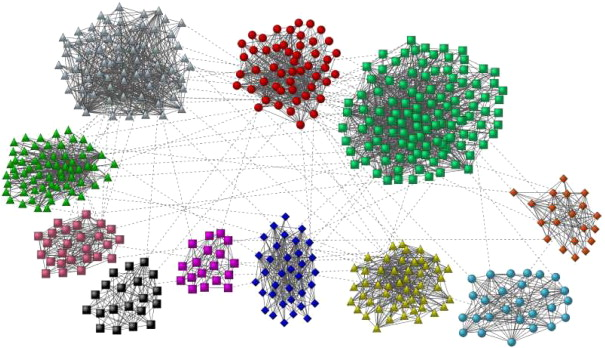
\includegraphics[width=1.0\linewidth]{images//communities.png}}
			\end{frame}
		
			\begin{frame}{Notations}

			\begin{block}{Assumption}
				We consider \textbf{undirected unweighted} graphs \textbf{without loops} with $n$ nodes.
				The nodes are enumerated as $\{ 1, ..., n\}$.\\
				Graph is given by its $n \times n $ adjacency matrix $A$.

			\end{block}

			\begin{block}{Goal of community detection}
				Find \textbf{partition} of nodes into \textbf{non-overlapping} clusters.\\
				The number of clusters is $k$.\\
				The clusters are denoted as $\{ \mathcal{C}_1, ..., \mathcal{C}_k\}$.
			\end{block}
		\end{frame}

	\section{Algorithms}
		\subsection{Spectral method}
			\begin{frame}{Subsets and Cuts}

\begin{block}{Measuring sizes of subsets}

Let $V_{1},\dots,V_{k}$ be subsets of vertices. Then:

\begin{itemize}

\item $|V_{i}| = \{\text{number of vertices in $V_{i}$}\}$

\item $vol(V_{i}) = \sum \limits_{i \in V_{i}}d_{i}$

\end{itemize}

\end{block}

\begin{block}{MinCut}

Define $W(S_1,S_2):= \sum \limits_{i \in S_1,j \in S_2}  a_{ij}.$ Then the MinCut problem is:

\[
cut(V_1,\dots,V_k) = \frac{1}{2}\sum\limits_{i=1}^kW(V_i,\overline{V_i}) \rightarrow \min \limits_{V_1,\dots,V_k}
\]
\end{block}

\end{frame}		

\begin{frame}{Balancing Cuts}

\begin{block}{RatioCut and Normalized Cut}

The MinCut solution separates one individual vertex from the rest. The following objectives are considered:

\[
RatioCut(V_1,\dots,V_k) = \sum \limits_{i=1}^k \frac{cut(V_i,\overline{V_i})}{|V_{i}|} \rightarrow \min \limits_{V_1,\dots,V_k}
\]

\[
Ncut(V_1,\dots,V_k)= \sum \limits_{i=1}^k \frac{cut(V_i,\overline{V_i})}{vol(V_{i})} \rightarrow \min \limits_{V_1,\dots,V_k}
\]

\end{block}

Balancing conditions lead to NP-hard problem. Spectral clustering is a way to solve relaxed versions of those problems

\end{frame}

\begin{frame}{Relaxed problem}

\begin{block}{Types of Laplacians}

\begin{itemize}

\item Unnormilized Laplacian: $L=D-A$

\item Symmetric Laplacian: $L_{sym} =D^{-\frac{1}{2}}LD^{-\frac{1}{2}}=I-D^{-\frac{1}{2}}AD^{-\frac{1}{2}}$

\item Random walk Laplacian: $L_{rw} =D^{-1}L=I-D^{-1}A$

\end{itemize}

\end{block}

\begin{block}{Idea}

\begin{itemize}

\item Solving relaxed problem is equivalent to considering eigenvectors corresponding to $k$ smallest eigenvalues of Laplacian that describe cluster properties of given graph

\end{itemize}

\end{block}

\begin{block}

\begin{itemize}
\item Ulrike von Luxburg <<A Tutorial on Spectral Clustering>>, 2007

\end{itemize}

\end{block}

\end{frame}

		\subsection{Modularity-based method}
			\begin{frame}{Modularity-based method}
				\begin{block}{Formulating an optimization problem}
				\end{block}
			\end{frame}

			\begin{frame}{Modularity-based method}
				
			\end{frame}
	
		\subsection{Conjugate gradients method}
			\begin{frame}{Conjugate gradients method}
				\begin{block}{Formulating an optimization problem}
				\end{block}
			\end{frame}

			\begin{frame}{Conjugate gradients method}
				
			\end{frame}

		\subsection{Semidefinite relaxations}
			\begin{frame}{Semidefinite relaxations}
				\begin{block}{Formulating an optimization problem}
				\end{block}
			\end{frame}

			\begin{frame}{Semidefinite relaxations}
				
			\end{frame}

	\section{Experimental results}
		\begin{frame}{}
				
		\end{frame}
\end{document}